\documentclass{standalone}
\usepackage{tikz}
\usetikzlibrary{patterns, positioning}
\usepackage[sfdefault]{ClearSans} %% option 'sfdefault' activates Clear Sans as the default text font
\usepackage[T1]{fontenc}

\begin{document}
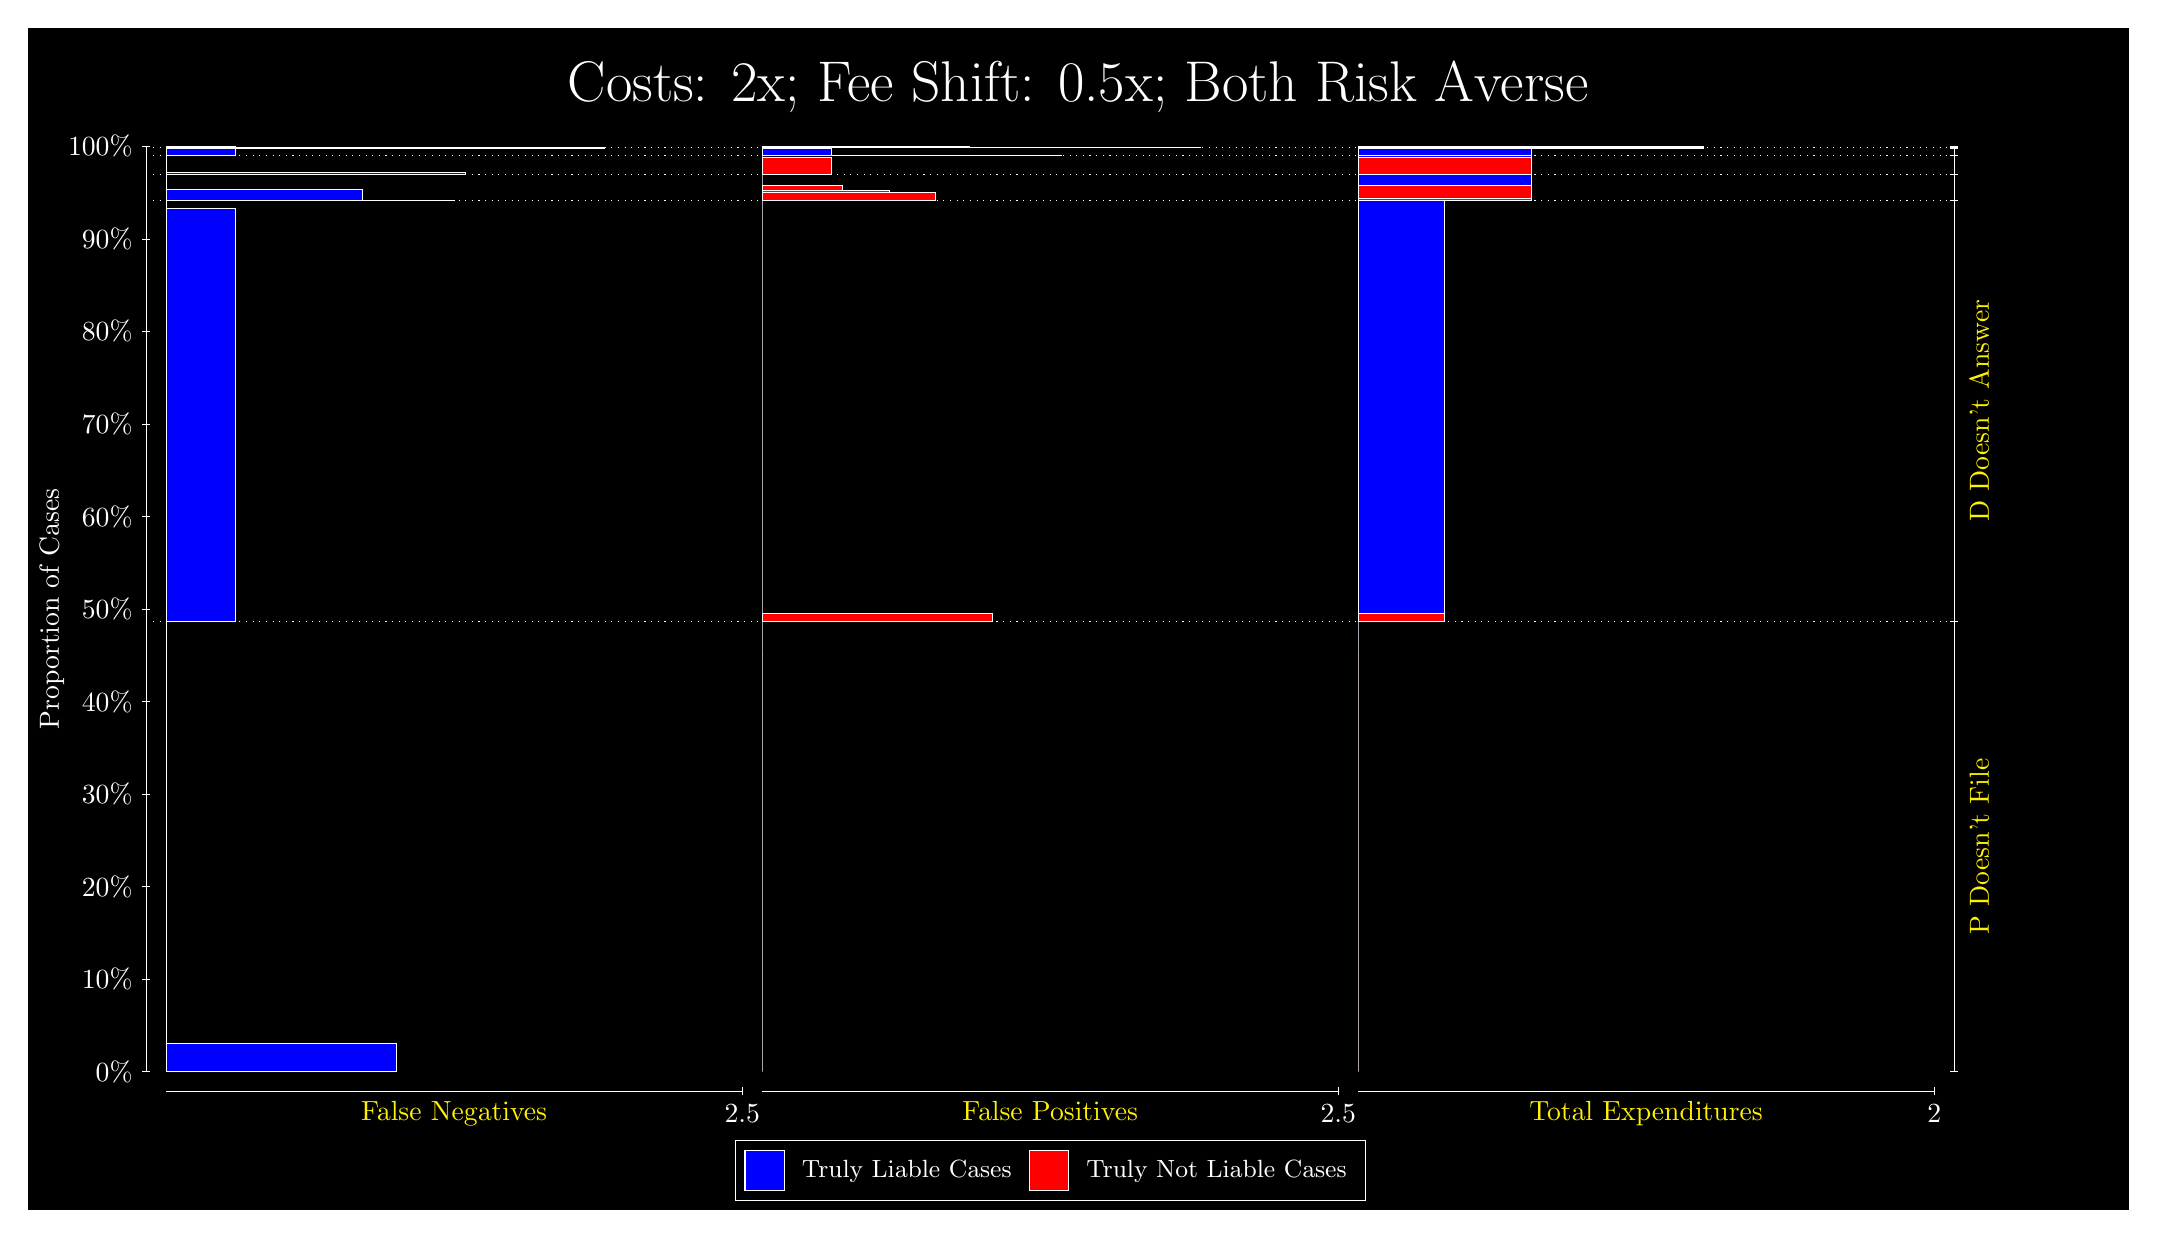
\begin{tikzpicture}
\draw[fill=black] (0,0) rectangle (26.667,15);
\draw[text=white] (0,13.5) rectangle (26.667,15) node[midway] {\huge Costs: 2x; Fee Shift: 0.5x; Both Risk Averse};
\draw[white, very thin] (1.5,1.75) -- (1.5,13.5);
\node[rotate=90, text=white, anchor=center] at (0.3, 7.625) {Proportion of Cases};
\draw[white, very thin] (1.45,1.75) -- (1.55,1.75);
\node[text=white, anchor=east] at (1.45, 1.75) {0\%};
\draw[white, very thin] (1.45,2.925) -- (1.55,2.925);
\node[text=white, anchor=east] at (1.45, 2.925) {10\%};
\draw[white, very thin] (1.45,4.1) -- (1.55,4.1);
\node[text=white, anchor=east] at (1.45, 4.1) {20\%};
\draw[white, very thin] (1.45,5.275) -- (1.55,5.275);
\node[text=white, anchor=east] at (1.45, 5.275) {30\%};
\draw[white, very thin] (1.45,6.45) -- (1.55,6.45);
\node[text=white, anchor=east] at (1.45, 6.45) {40\%};
\draw[white, very thin] (1.45,7.625) -- (1.55,7.625);
\node[text=white, anchor=east] at (1.45, 7.625) {50\%};
\draw[white, very thin] (1.45,8.8) -- (1.55,8.8);
\node[text=white, anchor=east] at (1.45, 8.8) {60\%};
\draw[white, very thin] (1.45,9.975) -- (1.55,9.975);
\node[text=white, anchor=east] at (1.45, 9.975) {70\%};
\draw[white, very thin] (1.45,11.15) -- (1.55,11.15);
\node[text=white, anchor=east] at (1.45, 11.15) {80\%};
\draw[white, very thin] (1.45,12.325) -- (1.55,12.325);
\node[text=white, anchor=east] at (1.45, 12.325) {90\%};
\draw[white, very thin] (1.45,13.5) -- (1.55,13.5);
\node[text=white, anchor=east] at (1.45, 13.5) {100\%};

\draw[white, very thin] (24.457,1.75) -- (24.457,13.5);
\draw[white, very thin] (24.407,1.75) -- (24.507,1.75);
\node[anchor=west] at (24.407, 1.75) {};
\draw[white, very thin] (24.407,7.4708) -- (24.507,7.4708);
\node[anchor=west] at (24.407, 7.4708) {};
\draw[white, very thin] (24.407,12.815) -- (24.507,12.815);
\node[anchor=west] at (24.407, 12.815) {};
\draw[white, very thin] (24.407,13.143) -- (24.507,13.143);
\node[anchor=west] at (24.407, 13.143) {};
\draw[white, very thin] (24.407,13.383) -- (24.507,13.383);
\node[anchor=west] at (24.407, 13.383) {};
\draw[white, very thin] (24.407,13.481) -- (24.507,13.481);
\node[anchor=west] at (24.407, 13.481) {};
\draw[white, very thin] (24.407,13.487) -- (24.507,13.487);
\node[anchor=west] at (24.407, 13.487) {};
\draw[white, very thin] (24.407,13.5) -- (24.507,13.5);
\node[anchor=west] at (24.407, 13.5) {};

\draw[white, very thin, fill=blue] (1.75,1.75) rectangle (4.6775,2.1093);
\draw[white, very thin, fill=red] (1.75,2.1093) rectangle (1.75,7.4708);
\draw[white, very thin, fill=blue] (1.75,7.4708) rectangle (2.6283,12.714);
\draw[white, very thin, fill=red] (1.75,12.714) rectangle (1.75,12.815);
\draw[white, very thin, fill=blue] (1.75,12.815) rectangle (5.4094,12.817);
\draw[white, very thin, fill=blue] (1.75,12.817) rectangle (4.8239,12.821);
\draw[white, very thin, fill=blue] (1.75,12.821) rectangle (4.2384,12.954);
\draw[white, very thin, fill=red] (1.75,12.954) rectangle (1.75,13.143);
\draw[white, very thin, fill=blue] (1.75,13.143) rectangle (5.5558,13.171);
\draw[white, very thin, fill=red] (1.75,13.171) rectangle (1.75,13.383);
\draw[white, very thin, fill=blue] (1.75,13.383) rectangle (2.6283,13.476);
\draw[white, very thin, fill=red] (1.75,13.476) rectangle (1.75,13.481);
\draw[white, very thin, fill=blue] (1.75,13.481) rectangle (7.3123,13.483);
\draw[white, very thin, fill=red] (1.75,13.483) rectangle (1.75,13.487);
\draw[white, very thin, fill=blue] (1.75,13.487) rectangle (2.6283,13.499);
\draw[white, very thin, fill=red] (1.75,13.499) rectangle (1.75,13.5);
\draw[white, very thin, fill=red] (9.3189,1.75) rectangle (9.3189,7.1115);
\draw[white, very thin, fill=blue] (9.3189,7.1115) rectangle (9.3189,7.4708);
\draw[white, very thin, fill=red] (9.3189,7.4708) rectangle (12.246,7.5723);
\draw[white, very thin, fill=blue] (9.3189,7.5723) rectangle (9.3189,12.815);
\draw[white, very thin, fill=red] (9.3189,12.815) rectangle (11.515,12.916);
\draw[white, very thin, fill=red] (9.3189,12.916) rectangle (10.929,12.94);
\draw[white, very thin, fill=red] (9.3189,12.94) rectangle (10.344,13.004);
\draw[white, very thin, fill=blue] (9.3189,13.004) rectangle (9.3189,13.143);
\draw[white, very thin, fill=red] (9.3189,13.143) rectangle (10.197,13.356);
\draw[white, very thin, fill=blue] (9.3189,13.356) rectangle (9.3189,13.383);
\draw[white, very thin, fill=red] (9.3189,13.383) rectangle (13.125,13.388);
\draw[white, very thin, fill=blue] (9.3189,13.388) rectangle (10.197,13.481);
\draw[white, very thin, fill=red] (9.3189,13.481) rectangle (10.197,13.485);
\draw[white, very thin, fill=blue] (9.3189,13.485) rectangle (9.3189,13.487);
\draw[white, very thin, fill=red] (9.3189,13.487) rectangle (14.881,13.488);
\draw[white, very thin, fill=blue] (9.3189,13.488) rectangle (11.954,13.5);
\draw[white, very thin, fill=red] (16.888,1.75) rectangle (16.888,7.1115);
\draw[white, very thin, fill=blue] (16.888,7.1115) rectangle (16.888,7.4708);
\draw[white, very thin, fill=red] (16.888,7.4708) rectangle (17.986,7.5723);
\draw[white, very thin, fill=blue] (16.888,7.5723) rectangle (17.986,12.815);
\draw[white, very thin, fill=red] (16.888,12.815) rectangle (19.083,12.839);
\draw[white, very thin, fill=blue] (16.888,12.839) rectangle (19.083,12.844);
\draw[white, very thin, fill=red] (16.888,12.844) rectangle (19.083,13.009);
\draw[white, very thin, fill=blue] (16.888,13.009) rectangle (19.083,13.143);
\draw[white, very thin, fill=red] (16.888,13.143) rectangle (19.083,13.356);
\draw[white, very thin, fill=blue] (16.888,13.356) rectangle (19.083,13.383);
\draw[white, very thin, fill=red] (16.888,13.383) rectangle (19.083,13.388);
\draw[white, very thin, fill=blue] (16.888,13.388) rectangle (19.083,13.481);
\draw[white, very thin, fill=red] (16.888,13.481) rectangle (21.279,13.485);
\draw[white, very thin, fill=blue] (16.888,13.485) rectangle (21.279,13.487);
\draw[white, very thin, fill=red] (16.888,13.487) rectangle (21.279,13.488);
\draw[white, very thin, fill=blue] (16.888,13.488) rectangle (21.279,13.5);
\draw[white, dotted] (1.5,7.4708) -- (24.457,7.4708);
\draw[white, dotted] (1.5,12.815) -- (24.457,12.815);
\draw[white, dotted] (1.5,13.143) -- (24.457,13.143);
\draw[white, dotted] (1.5,13.383) -- (24.457,13.383);
\draw[white, dotted] (1.5,13.481) -- (24.457,13.481);
\draw[white, dotted] (1.5,13.487) -- (24.457,13.487);
\draw[white, very thin] (1.75,1.5) -- (9.0689,1.5);
\node[text=yellow, anchor=north] at (5.4094, 1.5) {False Negatives};
\draw[white, very thin] (9.0689,1.45) -- (9.0689,1.55);
\node[text=white, anchor=north] at (9.0689, 1.45) {2.5};

\draw[white, very thin] (9.3189,1.5) -- (16.638,1.5);
\node[text=yellow, anchor=north] at (12.978, 1.5) {False Positives};
\draw[white, very thin] (16.638,1.45) -- (16.638,1.55);
\node[text=white, anchor=north] at (16.638, 1.45) {2.5};

\draw[white, very thin] (16.888,1.5) -- (24.207,1.5);
\node[text=yellow, anchor=north] at (20.547, 1.5) {Total Expenditures};
\draw[white, very thin] (24.207,1.45) -- (24.207,1.55);
\node[text=white, anchor=north] at (24.207, 1.45) {2};

\node[text=yellow, centered, rotate=90] at (24.777, 4.6104) {P Doesn't File};
\node[text=yellow, centered, rotate=90] at (24.777, 10.143) {D Doesn't Answer};






\draw (12.978300999999998,1.5) node[draw=none] (baseCoordinate) {};
\begin{scope}[align=center]
        \matrix[scale=0.5, draw=white, below=0.5cm of baseCoordinate, nodes={draw}, column sep=0.1cm]{
            \node[rectangle, draw, minimum width=0.5cm, minimum height=0.5cm, fill=blue] {}; &
            \node[draw=none, font=\small, text=white] (B) {Truly Liable Cases}; &
            \node[rectangle, draw, minimum width=0.5cm, minimum height=0.5cm, fill=red] {}; &
            \node[draw=none, font=\small, text=white] (B) {Truly Not Liable Cases}; \\
            };
\end{scope}

\end{tikzpicture}
\end{document}